% =====================================================================
% Proyecto Final — Defensa académica
% Introducción a la Ingeniería de Datos (DIA.04) — ITBA
% Compilar con XeLaTeX (Overleaf: Menú → Compiler → XeLaTeX) o con tectonic
% =====================================================================
\documentclass[aspectratio=169,10pt]{beamer}

\usepackage{fontspec}
\usepackage[sfdefault]{FiraSans}
\usepackage{polyglossia}
\setdefaultlanguage{spanish}
\usepackage{booktabs}
\usepackage{tabularx}
\usepackage{listings}
\usepackage{tikz}
\usetikzlibrary{positioning, arrows.meta, shapes.multipart, fit, calc}

% ------------------------------------------------------------- colores ITBA
\definecolor{itba}{HTML}{02568A}
\definecolor{itbaclaro}{HTML}{7FA9C8}
\definecolor{itbafondo}{HTML}{EAF1F7}
\definecolor{tinta}{HTML}{1F2933}
\definecolor{gris}{HTML}{8A949E}
\definecolor{alerta}{HTML}{C0392B}

% ------------------------------------------------------------- tema
\usetheme{default}
\setbeamertemplate{navigation symbols}{}
\setbeamercolor{normal text}{fg=tinta,bg=white}
\setbeamercolor{structure}{fg=itba}
\setbeamercolor{frametitle}{fg=itba,bg=white}
\setbeamercolor{alerted text}{fg=alerta}
\setbeamercolor{block title}{fg=white,bg=itba}
\setbeamercolor{block body}{fg=tinta,bg=itbafondo}
\setbeamerfont{frametitle}{size=\Large,series=\bfseries}
\setbeamertemplate{itemize item}{\color{itba}\rule[0.25ex]{0.9ex}{0.9ex}}
\setbeamertemplate{itemize subitem}{\color{itbaclaro}\rule[0.3ex]{0.7ex}{0.7ex}}
\setbeamertemplate{enumerate item}{\color{itba}\bfseries\insertenumlabel.}
\setbeamertemplate{blocks}[rounded][shadow=false]

\makeatletter
\setbeamertemplate{frametitle}{%
  \vspace*{0.35cm}%
  \begin{beamercolorbox}[wd=\paperwidth,leftskip=0.6cm]{frametitle}%
    \usebeamerfont{frametitle}\insertframetitle%
    \ifx\insertframesubtitle\@empty\else\\[-0.1ex]{\normalsize\color{gris}\mdseries\insertframesubtitle}\fi%
  \end{beamercolorbox}%
  \vspace*{-0.15cm}%
  {\color{itba}\hspace*{0.6cm}\rule{2.2cm}{2.5pt}}%
}
\makeatother
\setbeamertemplate{footline}{%
  \begin{tikzpicture}[remember picture, overlay]
    \fill[itba] (current page.south west) rectangle ([yshift=0.13cm]current page.south east);
  \end{tikzpicture}%
  \hspace*{0.6cm}{\scriptsize\color{gris}Marcos Kantor · Proyecto Final · Introducción a la Ingeniería de Datos}%
  \hfill\raisebox{-0.12cm}{
\includegraphics[height=0.42cm]{fig/logo_itba.png}}%
  \hspace*{0.35cm}{\scriptsize\color{itba}\bfseries\insertframenumber}\hspace*{0.6cm}\vspace*{0.3cm}%
}

\lstset{
  basicstyle=\ttfamily\footnotesize\color{tinta},
  keywordstyle=\color{itba}\bfseries,
  commentstyle=\color{gris}\itshape,
  stringstyle=\color{alerta},
  backgroundcolor=\color{itbafondo},
  frame=none, breaklines=true, columns=fullflexible, showstringspaces=false,
  xleftmargin=4pt, xrightmargin=4pt, aboveskip=2pt, belowskip=2pt,
}

\newcommand{\dato}[2]{\begin{minipage}[t]{2.6cm}\centering{\Huge\bfseries\color{itba}#1}\\[0.6ex]{\footnotesize\color{gris}#2}\end{minipage}}
% Separador de sección con indicador de ubicación (Fundamentos de storytelling, parte 2: «Ubicación»):
% la etapa actual en blanco y negrita, las demás en azul claro. \separador[n]{Título}; n = 0 no resalta ninguna.
\newcommand{\etapas}{Tablero,ETL,Calidad,OpenCV,BD transacc.,Almacén,Veredicto}
\newcommand{\separador}[2][0]{%
  {\setbeamertemplate{footline}{}
  \begin{frame}[plain]
    \begin{tikzpicture}[remember picture, overlay]
      \fill[itba] (current page.south west) rectangle (current page.north east);
      \node[anchor=west, text=white, font=\Huge\bfseries, text width=12cm] at ([xshift=1.2cm]current page.west) {#2};
      \fill[white] ([xshift=1.2cm,yshift=-0.9cm]current page.west) rectangle ++(2.2cm,0.08cm);
      \foreach \e [count=\i] in \etapas {%
        \ifnum\i=#1\relax
          \node[anchor=south west, text=white, font=\scriptsize\bfseries, inner sep=0pt]
            at ([xshift=1.2cm+(\i-1)*2.05cm, yshift=0.9cm]current page.south west) {\i.\,\e};
          \fill[white] ([xshift=1.2cm+(\i-1)*2.05cm, yshift=0.7cm]current page.south west) rectangle ++(1.8cm,0.06cm);
        \else
          \node[anchor=south west, text=itbaclaro, font=\scriptsize, inner sep=0pt]
            at ([xshift=1.2cm+(\i-1)*2.05cm, yshift=0.9cm]current page.south west) {\i.\,\e};
        \fi
      }
    \end{tikzpicture}
  \end{frame}}}

% ER / almacén
\tikzset{
  tabla/.style={rectangle split, rectangle split parts=2, draw=itba, line width=0.7pt, rounded corners=2pt,
                rectangle split part fill={itba,white}, font=\scriptsize, align=left, inner sep=3pt, text width=#1},
  tabla/.default=2.9cm,
  hechos/.style={tabla=#1, rectangle split part fill={alerta,white}, draw=alerta},
  rel/.style={-{Latex[length=1.6mm]}, draw=gris, line width=0.7pt},
}
\newcommand{\tab}[4][2.9cm]{\node[tabla=#1] (#2) at #3 {\textcolor{white}{\textbf{#2}}\nodepart{two}#4};}


\newcommand{\leer}[1]{\begin{block}{Cómo leerlo}\footnotesize #1\end{block}}
\newcommand{\dice}[1]{\setbeamercolor{block title}{fg=white,bg=alerta}\setbeamercolor{block body}{fg=tinta,bg=alerta!8}\begin{block}{Qué nos dice}\footnotesize #1\end{block}}
\title{¿Alcanzan los datos públicos de radiografías lumbares para entrenar el detector de vértebras de un CDSS de inestabilidad espinal?}
\author{Marcos Kantor}
\date{Proyecto Final — Defensa académica}

\begin{document}

% ===================================================================== portada
{\setbeamertemplate{footline}{}
\begin{frame}[plain]
  \begin{tikzpicture}[remember picture, overlay]
    \fill[itba] (current page.south west) rectangle ([yshift=2.2cm]current page.south east);
    \node[anchor=north west] at ([xshift=1cm,yshift=-0.8cm]current page.north west) {
\includegraphics[height=1.15cm]{fig/logo_itba.png}};
    \node[anchor=north west, text width=13.2cm, font=\LARGE\bfseries, text=itba, align=left]
      at ([xshift=1cm,yshift=-2.5cm]current page.north west) {\inserttitle};
    \node[anchor=north west, text width=13cm, font=\large, text=tinta]
      at ([xshift=1cm,yshift=-5.15cm]current page.north west) {Proyecto Final — Defensa académica};
    \node[anchor=west, text=white, font=\normalsize, align=left] at ([xshift=1cm,yshift=1.1cm]current page.south west)
      {\textbf{Marcos Kantor}\\[0.3ex]
       \footnotesize Director: Ramiro M. Irastorza (IFLySiB-CONICET)\\
       \footnotesize Codirector: Marcelo A. Cappelletti (LEICI-CONICET, UNAJ)};
    \node[anchor=north east, text=itba, font=\small, align=right] at ([xshift=-1cm,yshift=-0.85cm]current page.north east)
      {(20262Q) DIA.04\\Introducción a la Ingeniería de Datos\\Comisión A};
  \end{tikzpicture}
\end{frame}}

% ===================================================================== idea principal
\begin{frame}{La respuesta, antes que la evidencia}{Idea principal de la exposición}
  \vspace{0.6ex}
  {\setbeamercolor{block body}{fg=tinta,bg=itbafondo}
  \begin{block}{En una oración}
    \large Los datos públicos \textbf{alcanzan} para entrenar el detector de vértebras L1--L5 \textbf{sólo si se combinan dos fuentes}: NHANES aporta el volumen y Lumbar Spine la forma, la clínica y las vistas de frente. Antes hay que \textbf{\color{alerta}enderezar el 11\,\%} de NHANES.
  \end{block}}
  \vspace{1.2ex}
  \begin{center}
    \dato{\color{alerta}33}{completas en Lumbar Spine: no alcanza}\hspace{0.4cm}%
    \dato{4.405}{completas en NHANES}\hspace{0.4cm}%
    \dato{\color{alerta}477}{radiografías giradas o invertidas}\hspace{0.4cm}%
    \dato{36°}{de Cobb en escoliosis (7° en normales)}
  \end{center}
  \vspace{0.6ex}
  {\footnotesize\color{gris}Lo que sigue es la evidencia: extracción, calidad, modelado y tablero.}
\end{frame}

% ===================================================================== agenda
\begin{frame}{Recorrido de la exposición}
  \begin{columns}[T]
    \begin{column}{0.48\textwidth}
      \begin{enumerate}\setlength{\itemsep}{0.9ex}
        \item Pregunta de investigación y dataset
        \item \textbf{Demostración del tablero}
        \item Proceso de ETL
        \item Datos faltantes y anomalías
        \item \textbf{Descriptores de forma con OpenCV} y análisis exploratorio
        \item Modelo entidad-relación transaccional
        \item Diseño del almacén de datos
        \item Resultados y veredicto
      \end{enumerate}
    \end{column}
    \begin{column}{0.46\textwidth}
      \begin{block}{Artefactos (repositorio GitHub del curso)}
        \footnotesize
        \texttt{Proyecto\_final.ipynb} — Colab reproducible\\
        \texttt{spine\_oltp.db} — SQLite transaccional\\
        \texttt{spine\_dw.db} — SQLite almacén\\
        \texttt{app.py} — tablero Streamlit\\
        \texttt{data/raw/…zip} — dato crudo (CC BY 4.0)
      \end{block}
      \vspace{1ex}
      {\footnotesize\color{gris}Se ejecuta con \emph{Entorno de ejecución → Ejecutar todo}, sin credenciales ni archivos subidos a mano.}
    \end{column}
  \end{columns}
\end{frame}

% ===================================================================== pregunta
\begin{frame}{La pregunta}
  \begin{columns}[T]
    \begin{column}{0.4\textwidth}
      \small
      El \textbf{SINS} (\emph{Spinal Instability Neoplastic Score}) se evalúa \textbf{vértebra por vértebra}: localización, alineación, colapso, compromiso posterior.\\[1ex]
      La primera etapa de un CDSS que lo asista es \textbf{encontrar y delimitar cada vértebra}.\\[1.5ex]
      \begin{block}{Pregunta de investigación}
        \footnotesize ¿El dataset público \emph{Lumbar Spine} tiene la cobertura, el balance, la calidad geométrica y la coherencia anatómica necesarias para entrenar el detector L1–L5?
      \end{block}
    \end{column}
    \begin{column}{0.56\textwidth}
      \footnotesize
      \renewcommand{\arraystretch}{1.35}
      \begin{tabularx}{\linewidth}{@{}lX@{}}
        \toprule
        & \textbf{Preguntas de análisis} (guían el almacén y el tablero) \\
        \midrule
        \textbf{\color{itba}P1} & \textbf{Cobertura y balance:} ¿cuántas imágenes tienen L1–L5 completas? ¿están balanceadas las clases? ¿Y sumando una segunda fuente? \\
        \textbf{\color{itba}P2} & \textbf{Calidad geométrica:} ¿qué anotaciones tienen tamaño o forma atípicos para su vértebra? \\
        \textbf{\color{itba}P3} & \textbf{Coherencia anatómica:} ¿se respeta el orden L1$\rightarrow$L5 y el aumento de tamaño hacia caudal? \\
        \textbf{\color{itba}P4} & \textbf{Representatividad:} ¿qué diagnósticos, sexos y edades cubre? \\
        \textbf{\color{itba}P5} & \textbf{Alineación:} ¿la inclinación y el desplazamiento medidos con momentos de imagen distinguen las patologías? \\
        \bottomrule
      \end{tabularx}
    \end{column}
  \end{columns}
\end{frame}

% ===================================================================== dataset
\begin{frame}{Lumbar Spine: pocos datos, con contornos y clínica}{rp-team, Roboflow Universe, versión 1, licencia CC BY 4.0}
  \begin{columns}[c]
    \begin{column}{0.27\textwidth}
      \centering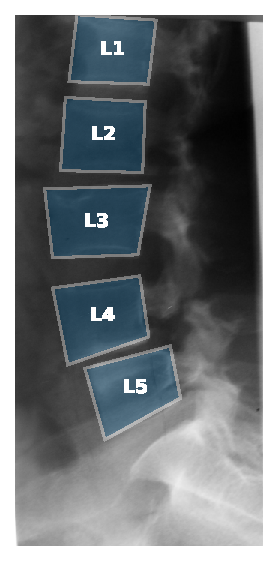
\includegraphics[height=5.5cm]{fig/radiografia.pdf}
    \end{column}
    \begin{column}{0.7\textwidth}
      \begin{center}
        \dato{50}{radiografías}\dato{34}{anotadas}\dato{170}{polígonos}\dato{5}{clases L1–L5}
      \end{center}
      \vspace{0.8ex}
      \small
      \begin{itemize}\setlength{\itemsep}{0.3ex}
        \item Polígonos: cada línea es \texttt{clase x1 y1 … xn yn} en $[0,1]$.
        \item De \textbf{144$\times$725} a \textbf{1669$\times$3246} px: recortes lumbares y columnas completas.
        \item El \textbf{nombre de archivo codifica datos clínicos}:\\[0.4ex]
          {\footnotesize\texttt{N18-\textcolor{itba}{Olisthesis}-L4-5-\textcolor{itba}{F}-\textcolor{itba}{56}-Yrs\_jpg.rf.<hash>.jpg}}\\[0.2ex]
          {\footnotesize diagnóstico · sexo · edad $\Rightarrow$ expresiones regulares (P4).}
        \item La espondilolistesis es pertinente para el criterio de \textbf{alineación} del SINS.
      \end{itemize}
    \end{column}
  \end{columns}
\end{frame}

\begin{frame}{NHANES multiplica el volumen, pero con cajas y de perfil}{Segunda fuente para responder P1, P3 y el veredicto}
  \begin{columns}[T]
    \begin{column}{0.5\textwidth}
      \begin{center}
        \dato{4.436}{radiografías de perfil}\dato{22.185}{cajas L1–L5}
      \end{center}
      \small
      \begin{itemize}\setlength{\itemsep}{0.5ex}
        \item Radiografías lumbares de la encuesta nacional de salud \textbf{NHANES} (EE.\,UU.), anotadas en Roboflow Universe (\texttt{main-kybbe}), \textbf{CC BY 4.0}.
        \item Anotadas con \textbf{cajas}, no polígonos, y estiradas a 640$\times$640 por la fuente.
        \item Se publica en GitHub \textbf{sólo la anotación COCO} (542 KB): P1 necesita qué vértebras hay, no los píxeles.
      \end{itemize}
    \end{column}
    \begin{column}{0.46\textwidth}
      \begin{block}{Qué responde y qué no}
        \footnotesize
        \textbf{Sí:} P1 (cobertura y veredicto) y P3 (orden y orientación).\\[0.4ex]
        \textbf{No:} P2 y P5. Una caja alineada con los ejes no tiene forma ni inclinación; P4 tampoco, porque no trae metadatos clínicos.
      \end{block}
      \vspace{0.6ex}
      \footnotesize\color{gris}Se integra al mismo modelo: nueva fila en \texttt{dataset}, \texttt{imagen.dataset\_id} y \texttt{anotacion.geometria} = \texttt{caja}.
    \end{column}
  \end{columns}
\end{frame}

% ===================================================================== demo
\separador[1]{Demostración del tablero}

\begin{frame}{El tablero responde primero: con dos fuentes, alcanza}{Streamlit · lee sólo del almacén \texttt{spine\_dw.db} · en Colab se abre al final del notebook}
  \centering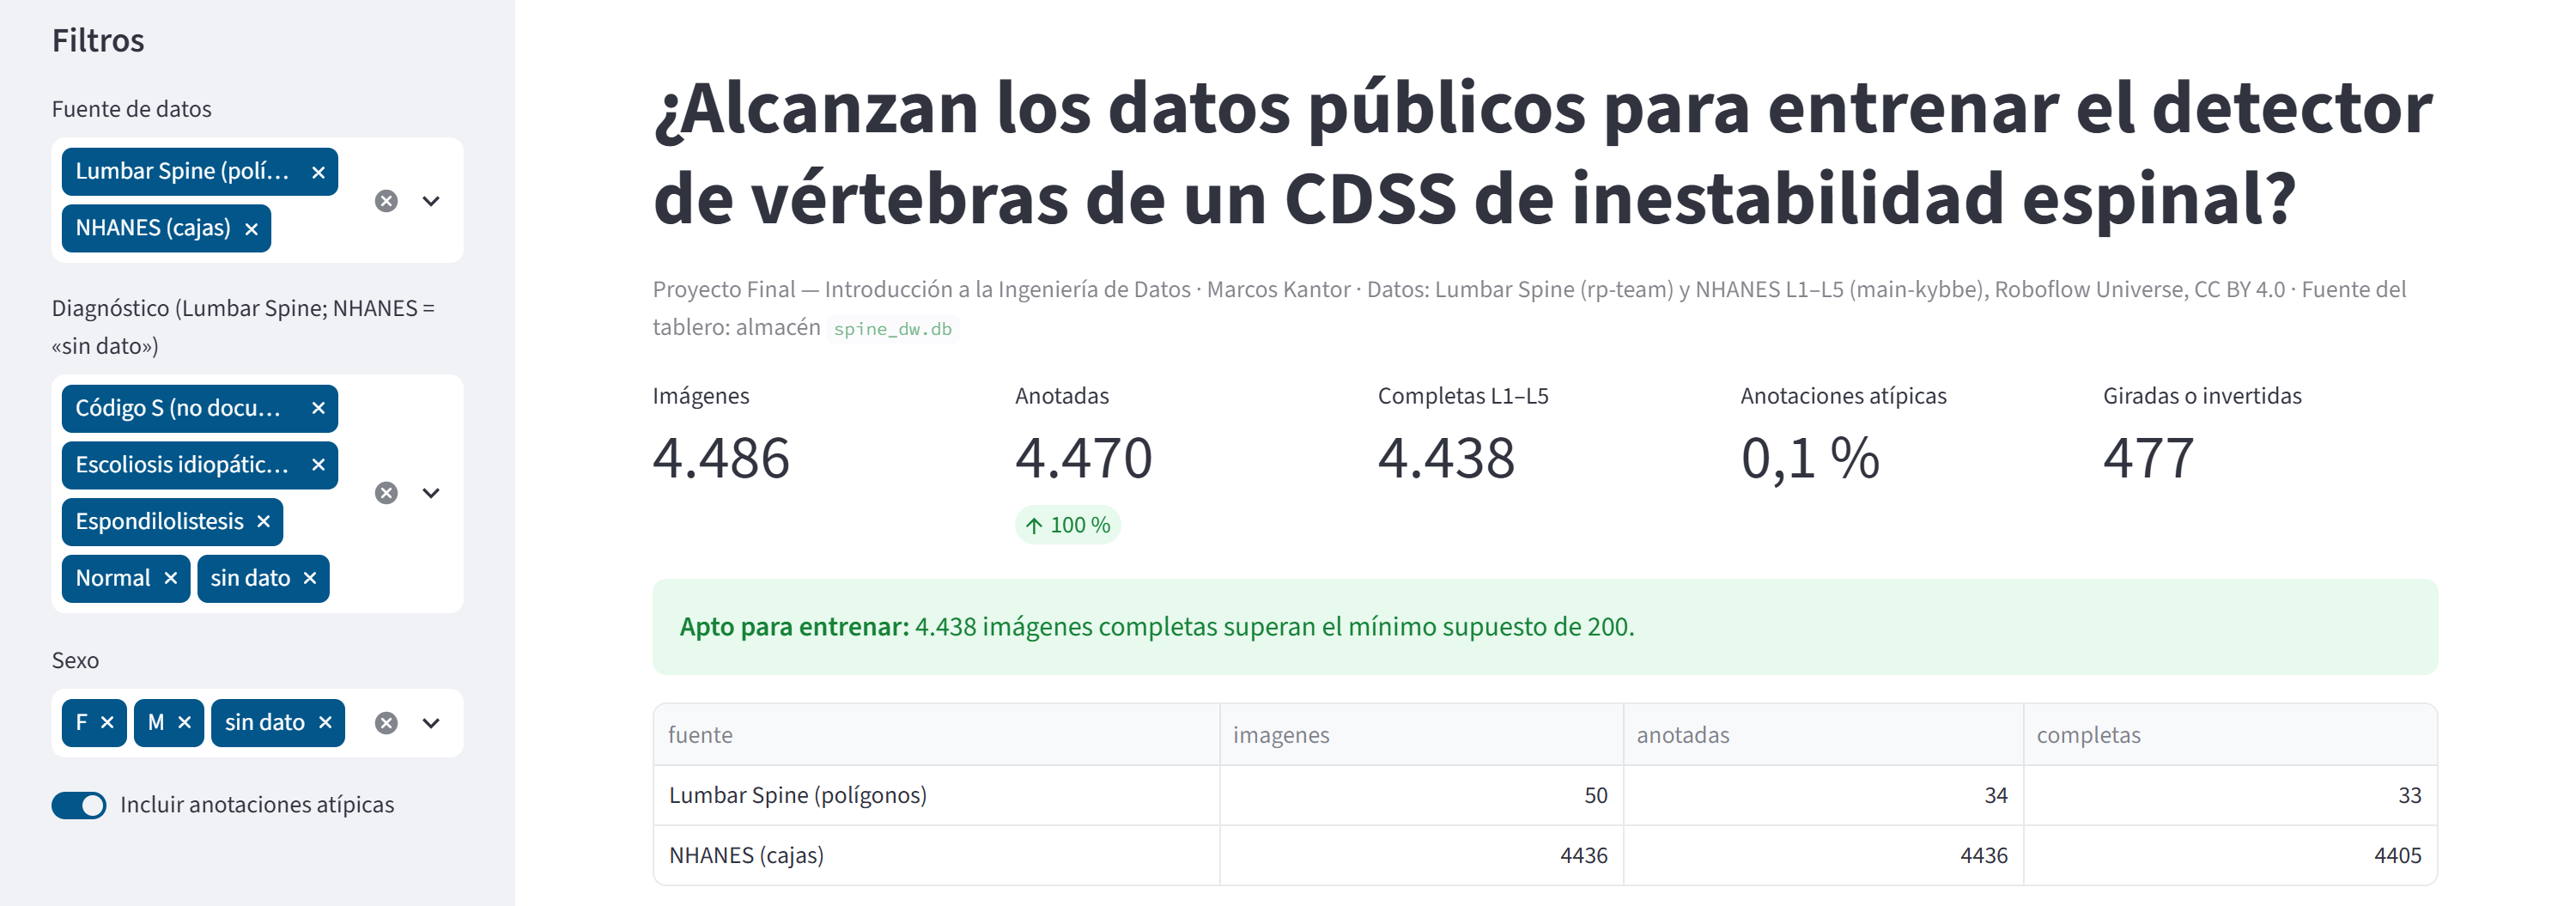
\includegraphics[width=0.74\linewidth]{fig/tablero_principal.png}\\[0.4ex]
  \begin{columns}[T]
    \begin{column}{0.48\textwidth}
      \leer{Arriba, la pregunta. Debajo, cinco indicadores, un \textbf{veredicto en color} (rojo = no alcanza, amarillo = ajuste fino, verde = apto) y la tabla por fuente.}
    \end{column}
    \begin{column}{0.48\textwidth}
      \dice{Con las dos fuentes hay \textbf{4.438 imágenes completas}: apto. Si se deja sólo Lumbar Spine (filtro «Fuente»), vuelve el rojo: 33 no alcanzan. El mínimo (200) es un supuesto ajustable.}
    \end{column}
  \end{columns}
\end{frame}

\begin{frame}{P1 · Lumbar Spine sola no alcanza: 33 imágenes completas}{Tablero · ¿cuántas imágenes tienen L1–L5 completas?}
  \begin{columns}[T]
    \begin{column}{0.33\textwidth}
      \centering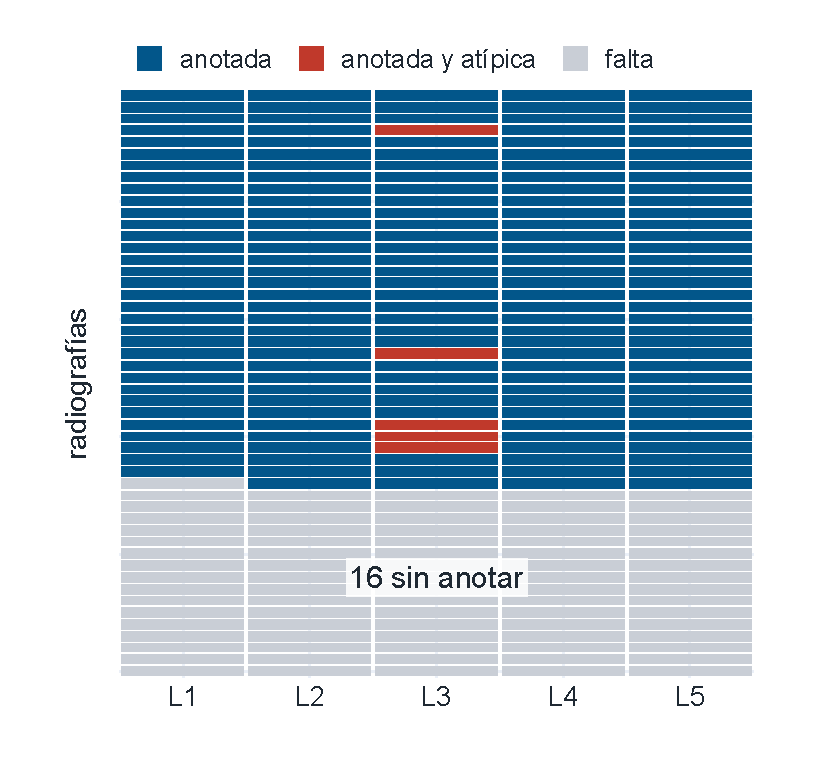
\includegraphics[height=5.2cm]{fig/tab_cobertura.pdf}
    \end{column}
    \begin{column}{0.41\textwidth}
      \centering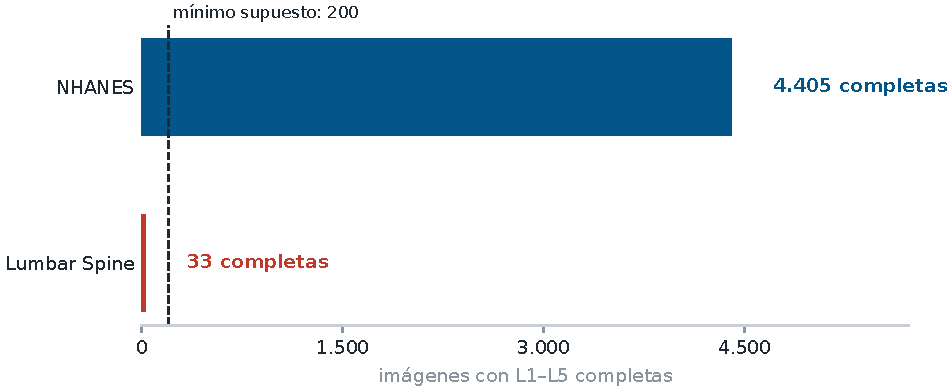
\includegraphics[width=\linewidth]{fig/tab_fuentes.pdf}\\[-0.5ex]
      {\scriptsize Imágenes completas por fuente}
    \end{column}
    \begin{column}{0.25\textwidth}
      \leer{Izquierda (Lumbar Spine): \textbf{cada fila es una radiografía}; azul = anotada, rojo = atípica, gris = falta. Derecha: completas por fuente y el mínimo.}
      \dice{Lumbar Spine: 33 completas y \textbf{16 sin anotar}. NHANES: \textbf{4.405}. Sumadas superan el mínimo.}
    \end{column}
  \end{columns}
\end{frame}

\begin{frame}{P3 · La anatomía se respeta; el problema es la orientación}{Tablero · ¿las anotaciones respetan el orden L1→L5?}
  \begin{columns}[T]
    \begin{column}{0.37\textwidth}
      \centering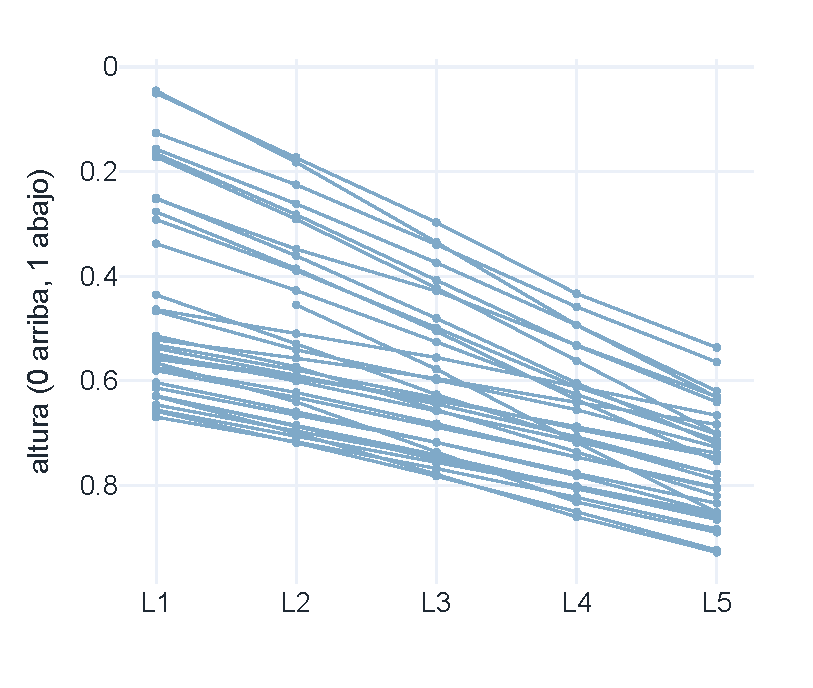
\includegraphics[width=\linewidth]{fig/tab_orden.pdf}\\[-0.3ex]
      {\scriptsize Posición de cada vértebra en su radiografía}
    \end{column}
    \begin{column}{0.37\textwidth}
      \centering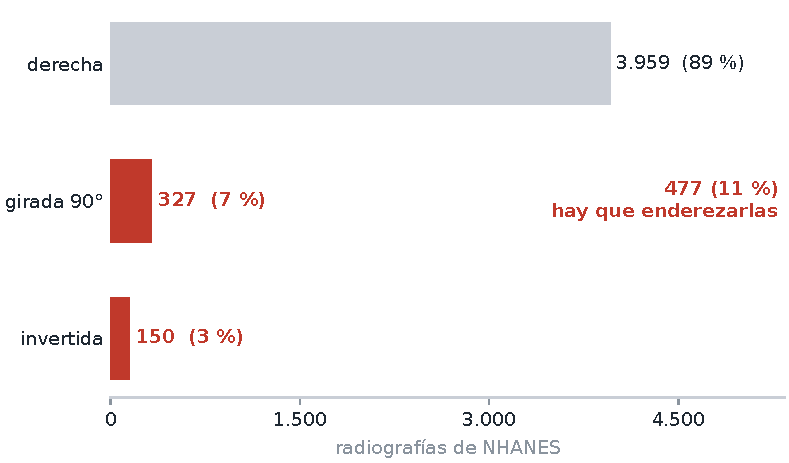
\includegraphics[width=\linewidth]{fig/tab_orientacion.pdf}\\[-0.3ex]
      {\scriptsize Orientación de las radiografías}
    \end{column}
    \begin{column}{0.24\textwidth}
      \leer{Izquierda (Lumbar Spine): \textbf{cada línea es una radiografía}; debe bajar de L1 a L5. Derecha (NHANES): en rojo, las que hay que enderezar.}
      \dice{Lumbar Spine: 0 errores. NHANES: \textbf{477 giradas o invertidas} (11\,\%) y sólo 26 cajas mal etiquetadas.}
    \end{column}
  \end{columns}
\end{frame}

\begin{frame}{P2 · Sólo 5 de 169 contornos son atípicos}{Tablero · ¿hay anotaciones mal dibujadas?}
  \begin{columns}[T]
    \begin{column}{0.66\textwidth}
      \centering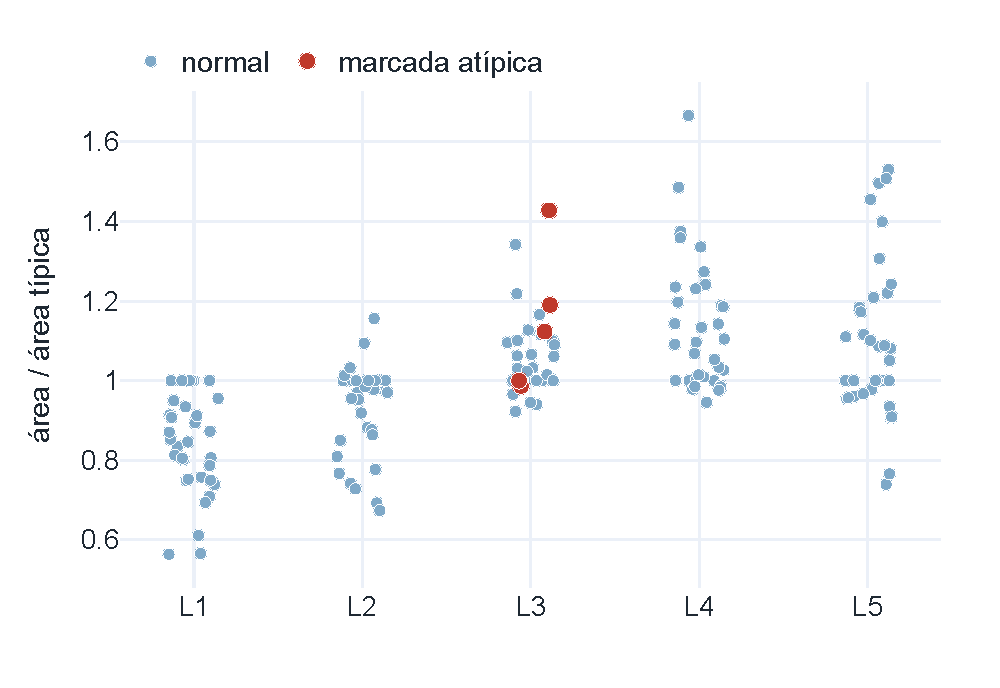
\includegraphics[width=\linewidth]{fig/tab_calidad.pdf}
    \end{column}
    \begin{column}{0.32\textwidth}
      \leer{\textbf{Cada punto es una vértebra anotada.} 1 = mismo tamaño que las otras vértebras de su radiografía. En rojo, las que el control estadístico marcó como atípicas.}
      \dice{Sólo \textbf{5 de 169}, todas L3. No se borran: el tablero las lista con su motivo para \textbf{revisarlas a mano}.}
    \end{column}
  \end{columns}
\end{frame}

\begin{frame}{P4 y P5 · Faltan escoliosis, pero el contorno mide la curva}{Tablero · ¿qué cubre el dataset y qué se puede medir?}
  \begin{columns}[T]
    \begin{column}{0.37\textwidth}
      \centering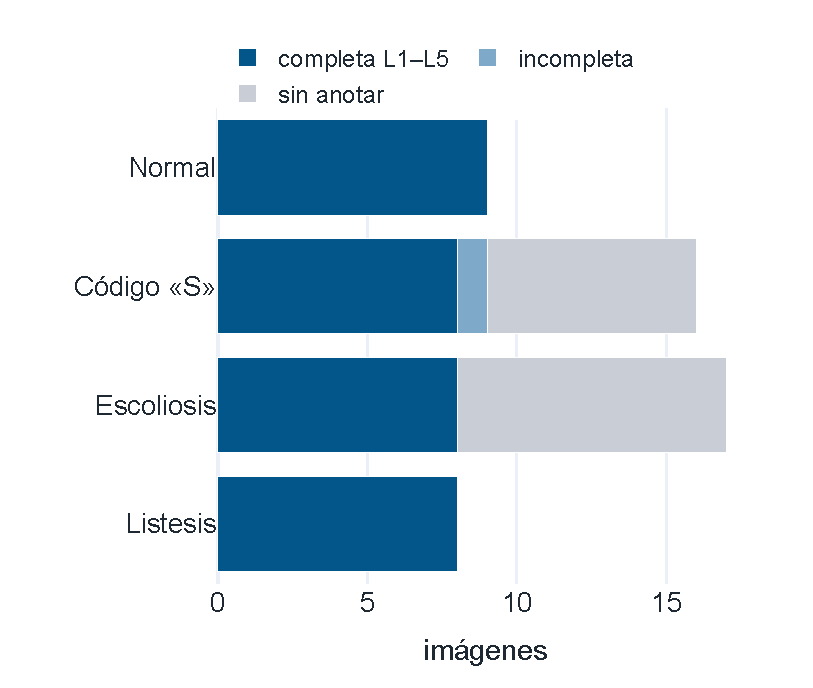
\includegraphics[width=\linewidth]{fig/tab_diagnostico.pdf}\\[-0.3ex]
      {\scriptsize P4 · Imágenes por diagnóstico}
    \end{column}
    \begin{column}{0.37\textwidth}
      \centering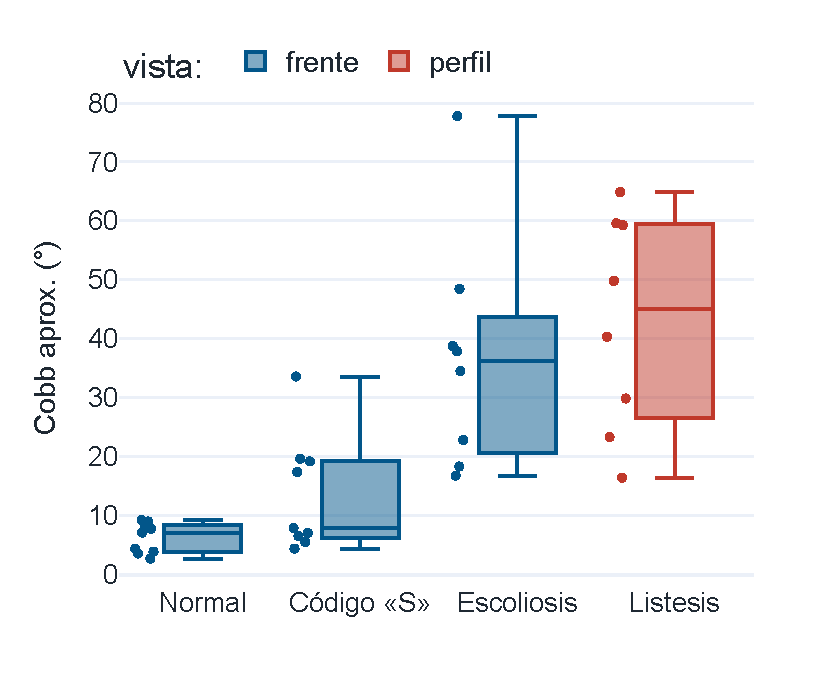
\includegraphics[width=\linewidth]{fig/tab_cobb.pdf}\\[-0.3ex]
      {\scriptsize P5 · Cobb aproximado por radiografía}
    \end{column}
    \begin{column}{0.24\textwidth}
      \leer{Izquierda: azul = completa, rojo = sin anotar. Derecha: \textbf{cada punto es una radiografía}; cuanto más alto, más inclinadas entre sí están sus vértebras.}
      \dice{Las sin anotar son escoliosis y «S». Escoliosis: \textbf{36°}; normales: \textbf{7°}. La curva se mide desde el contorno.}
    \end{column}
  \end{columns}
\end{frame}

% ===================================================================== ETL
\separador[2]{Proceso de ETL}

\begin{frame}{De dos zips públicos a un tablero, sin credenciales}{Pipeline de extracción, transformación y carga}
  \centering
  \begin{tikzpicture}[
      paso/.style={draw=itba, fill=itbafondo, rounded corners=3pt, line width=0.8pt, minimum height=1.05cm,
                   text width=2.15cm, align=center, font=\scriptsize},
      fase/.style={font=\scriptsize\bfseries, text=itba},
      flecha/.style={-{Latex[length=2mm]}, draw=itba, line width=0.9pt}]
    \node[paso] (e1) {2 zips crudos en GitHub\\\textbf{SHA-256}};
    \node[paso, right=0.45cm of e1] (e2) {Inventario por imagen\\+ metadatos};
    \node[paso, right=0.45cm of e2] (e3) {Parsing de polígonos\\(Gauss)};
    \node[paso, right=0.45cm of e3] (e4) {Staging CSV\\anotaciones, vértices};
    \node[paso, below=1.2cm of e4] (t1) {Carga optimizada\\\texttt{usecols} + tipos};
    \node[paso, left=0.45cm of t1] (t2) {Faltantes y duplicados};
    \node[paso, left=0.45cm of t2] (t3) {Atípicos y coherencia anatómica};
    \node[paso, left=0.45cm of t3] (t4) {Momentos OpenCV y variables sin escala};
    \node[paso, below=1.2cm of t4, fill=itba, text=white] (c1) {SQLite transaccional (3FN)};
    \node[paso, right=0.45cm of c1, fill=itba, text=white] (c2) {SQLite almacén (copo de nieve)};
    \node[paso, right=0.45cm of c2, fill=itba, text=white] (c3) {Tablero Streamlit};
    \node[paso, right=0.45cm of c3, draw=gris, fill=white] (c4) {Respuestas P1–P4 en SQL};
    \draw[flecha] (e1)--(e2); \draw[flecha] (e2)--(e3); \draw[flecha] (e3)--(e4); \draw[flecha] (e4)--(t1);
    \draw[flecha] (t1)--(t2); \draw[flecha] (t2)--(t3); \draw[flecha] (t3)--(t4); \draw[flecha] (t4)--(c1);
    \draw[flecha] (c1)--(c2); \draw[flecha] (c2)--(c3); \draw[flecha] (c2) to[bend right=25] (c4);
    \node[fase, left=0.25cm of e1, rotate=90, anchor=south] {Extracción};
    \node[fase, left=0.25cm of t4, rotate=90, anchor=south] {Transformación};
    \node[fase, left=0.25cm of c1, rotate=90, anchor=south] {Carga};
  \end{tikzpicture}
\end{frame}

\begin{frame}{Extracción verificada; carga con 88\,\% menos memoria}
  \begin{columns}[T]
    \begin{column}{0.5\textwidth}
      \textbf{\color{itba}Extracción sin credenciales}\\[0.6ex]
      \small
      \begin{itemize}\setlength{\itemsep}{0.5ex}
        \item Roboflow exige cuenta y API key $\Rightarrow$ no es \emph{estrictamente reproducible}.
        \item La licencia \textbf{CC BY 4.0} permite redistribuir: el zip crudo se publicó \textbf{sin modificar} en \texttt{data/raw/}.
        \item Descarga por URL pública + verificación \textbf{SHA-256}: todos obtienen los mismos bytes.
        \item Proceso \textbf{idempotente}: si el archivo está y el hash coincide, no se vuelve a bajar.
        \item El SDK de Roboflow queda como alternativa opcional.
      \end{itemize}
    \end{column}
    \begin{column}{0.47\textwidth}
      \textbf{\color{itba}Elección de columnas y tipado}\\[0.6ex]
      \footnotesize
      \begin{tabular}{@{}ll@{}}
        \toprule
        Variable & Tipo \\ \midrule
        \texttt{clase\_id}, \texttt{linea} & \texttt{int8} \\
        \texttt{ancho\_px}, \texttt{n\_vertices} & \texttt{int16} \\
        \texttt{edad} (puede faltar) & \texttt{Int8} \emph{nullable} \\
        coordenadas, áreas & \texttt{float32} \\
        \texttt{archivo}, \texttt{split}, \texttt{sexo} & \texttt{category} \\ \bottomrule
      \end{tabular}\\[1.2ex]
      \begin{tabular}{@{}lrr@{}}
        \toprule
        Tabla de staging & Filas & Ahorro \\ \midrule
        imágenes & 50 & 67\,\% \\
        anotaciones & 170 & 71\,\% \\
        vértices & 681 & 88\,\% \\ \bottomrule
      \end{tabular}\\[0.8ex]
      {\scriptsize\color{alerta}Ojo: \texttt{ancho*alto} en \texttt{int16} se desborda $\Rightarrow$ \texttt{float} antes de multiplicar.}
    \end{column}
  \end{columns}
\end{frame}

% ===================================================================== calidad
\separador[3]{Datos faltantes y anomalías}

\begin{frame}{Faltantes no aleatorios: 16 sin anotar, todas AIS o «S»}{Valores faltantes en cuatro niveles}
  \begin{columns}[T]
    \begin{column}{0.46\textwidth}
      \scriptsize
      \renewcommand{\arraystretch}{1.2}
      \begin{tabularx}{\linewidth}{@{}p{1.2cm}Xp{2cm}@{}}
        \toprule
        Nivel & Qué falta & Decisión \\ \midrule
        Imagen & 16 de 50 sin anotaciones & \textbf{se conservan} con \texttt{anotada = 0} \\
        Vértebra & imagen anotada sin alguna de L1–L5 & se mide la \textbf{completitud} \\
        Atributo & coordenadas o clase inválidas (0 casos) & \textbf{descarte} \\
        Metadato & sexo no identificable (1 imagen) & \textbf{nulo}, sin imputar \\ \bottomrule
      \end{tabularx}\\[1.2ex]
      \small
      \textbf{No se imputa geometría:} una vértebra inventada contamina el entrenamiento. \textbf{No se imputan datos clínicos:} inventaría pacientes y sesgaría P4.
    \end{column}
    \begin{column}{0.52\textwidth}
      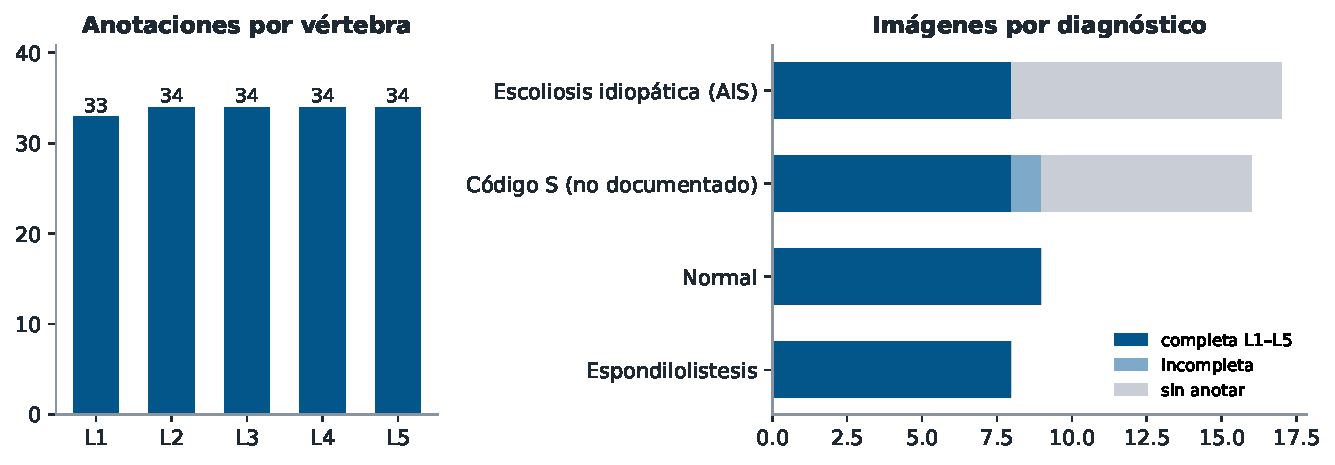
\includegraphics[width=\linewidth]{fig/cobertura.pdf}\\[0.5ex]
      \begin{block}{Hallazgo}
        \footnotesize Las 16 imágenes sin anotar son \textbf{todas} de escoliosis (9) o del código «S» (7): el faltante \textbf{no es aleatorio} (MNAR). Descartarlas sin registrarlo ocultaría un sesgo de cobertura.
      \end{block}
    \end{column}
  \end{columns}
\end{frame}

\begin{frame}{Se descarta sólo lo imposible: 1 duplicado y 0 inválidos}{Duplicados e inválidos geométricos}
  \begin{columns}[T]
    \begin{column}{0.5\textwidth}
      \textbf{\color{itba}Duplicados}\\[0.5ex]
      \small
      El grano esperado es \textbf{una anotación por (imagen, vértebra)}. En \texttt{N20-S-79-F} la \textbf{L2 aparece dos veces}.\\[0.8ex]
      \textbf{Regla:} se conserva la que está más cerca de la posición vertical mediana de L2 en todo el dataset.\\[0.6ex]
      \footnotesize
      \begin{tabular}{@{}lrrl@{}}
        \toprule
        Línea & $c_y$/alto & dist. a mediana & \\ \midrule
        3 & 0{,}455 & 0{,}118 & \textbf{se conserva} \\
        4 & 0{,}345 & 0{,}229 & descarte \\ \bottomrule
      \end{tabular}\\[0.6ex]
      \small Resultado: 170 $\rightarrow$ \textbf{169} anotaciones; la imagen queda incompleta (4 vértebras).
    \end{column}
    \begin{column}{0.47\textwidth}
      \textbf{\color{itba}Reglas de dominio}\\[0.5ex]
      \small
      \begin{itemize}\setlength{\itemsep}{0.5ex}
        \item Polígono fuera de la imagen más de un 2\,\% $\Rightarrow$ \textbf{descarte}.
        \item Desborde menor (redondeo del anotador) $\Rightarrow$ \textbf{recorte} al borde.
        \item Área $<$ 1 px$^2$ o menos de 3 vértices $\Rightarrow$ \textbf{descarte}.
      \end{itemize}
      \vspace{0.5ex}
      Resultado: \textbf{0 casos}; quedan como control para futuras versiones.\\[0.8ex]
      {\color{itba}\textbf{Criterio:} se descarta sólo lo imposible; lo raro se marca.}
    \end{column}
  \end{columns}
\end{frame}

\begin{frame}{Atípicos (1): la variable equivocada inventa 49 atípicos}{El área relativa a la imagen depende del encuadre; la relativa a sus vecinas, no}
  \centering
  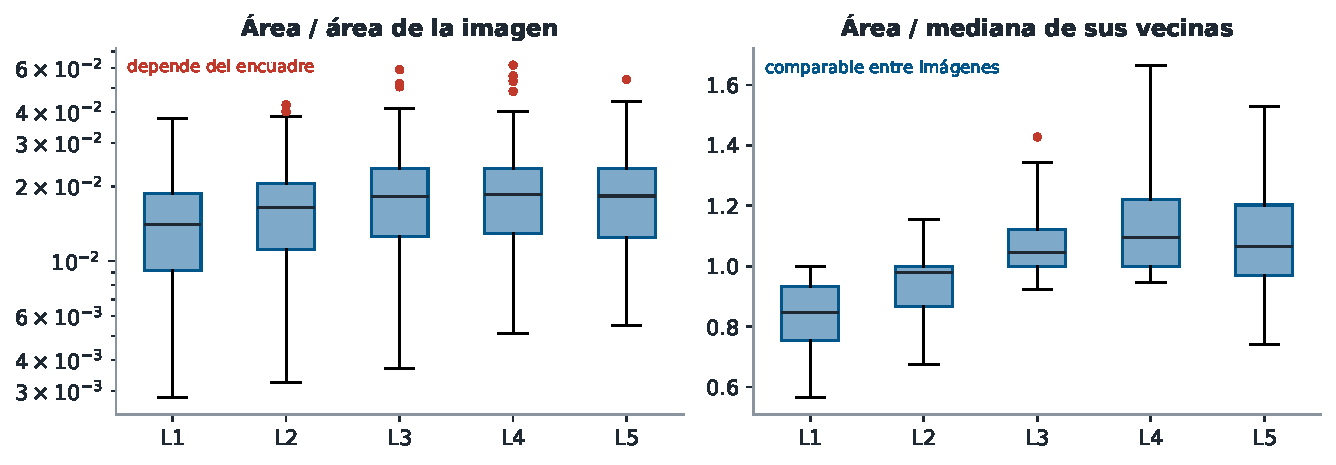
\includegraphics[height=3.9cm]{fig/encuadre.pdf}\\[0.4ex]
  \begin{columns}[T]
    \begin{column}{0.47\textwidth}
      \small
      \textbf{Primer intento:} área / área de la imagen.\\
      Marcó \textcolor{alerta}{\textbf{49 de 169}} anotaciones: \emph{imágenes enteras}, porque una es un recorte lumbar y otra una columna completa.
    \end{column}
    \begin{column}{0.47\textwidth}
      \small
      \textbf{Decisión:} normalizar \textbf{dentro de cada imagen}:\\
      \texttt{area\_norm} = área / mediana del área de sus vecinas.\\
      Atípicos: \textbf{\color{itba}5 de 169} — una vértebra es rara si no se parece a sus vecinas.
    \end{column}
  \end{columns}
\end{frame}

\begin{frame}{Atípicos (2): sin normalidad, Tukey y Mahalanobis robusta}
  \begin{columns}[T]
    \begin{column}{0.47\textwidth}
      \small
      Variables por vértebra: \texttt{area\_norm}, \texttt{aspecto} (ancho/alto), \texttt{relleno} (área del polígono / área de la caja).
      \begin{enumerate}\setlength{\itemsep}{0.6ex}
        \item \textbf{Shapiro–Wilk} por vértebra (n $\approx$ 34): \textbf{10 de 15} combinaciones \textbf{no} son normales ($\alpha$ = 0{,}05).
        \item $\Rightarrow$ el corte $|z| > 3$ no tiene sustento: se usan \textbf{Tukey fences} $Q_3 + 2\cdot\mathrm{RIC}$.
        \item \textbf{Mahalanobis robusta} (mediana y MAD) sobre las 3 variables: límite $\chi^2_{0{,}999}(3) = 16{,}27$; detecta combinaciones raras.
      \end{enumerate}
      \textbf{Decisión:} se \textbf{marcan} con su motivo; no se descartan.
    \end{column}
    \begin{column}{0.5\textwidth}
      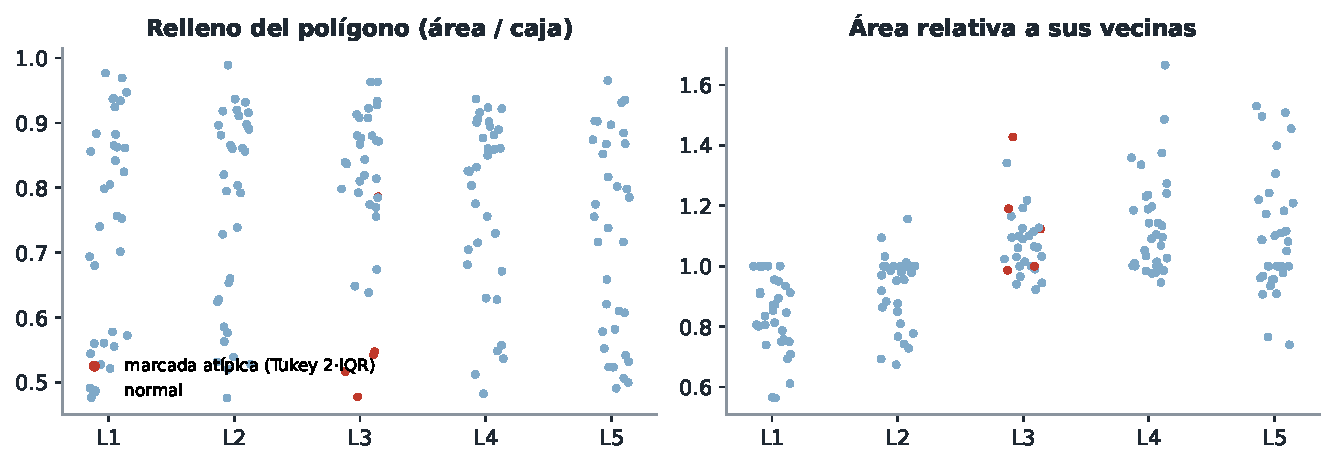
\includegraphics[width=\linewidth]{fig/atipicos.pdf}\\[0.5ex]
      \footnotesize Los 5 marcados son L3: 4 por \textbf{relleno bajo} (contorno poco ajustado al cuerpo vertebral) y 1 por \textbf{área alta} respecto de sus vecinas. Van a \textbf{revisión manual}.
    \end{column}
  \end{columns}
\end{frame}

\begin{frame}{Anatomía coherente: 0 errores de orden}
  \centering
  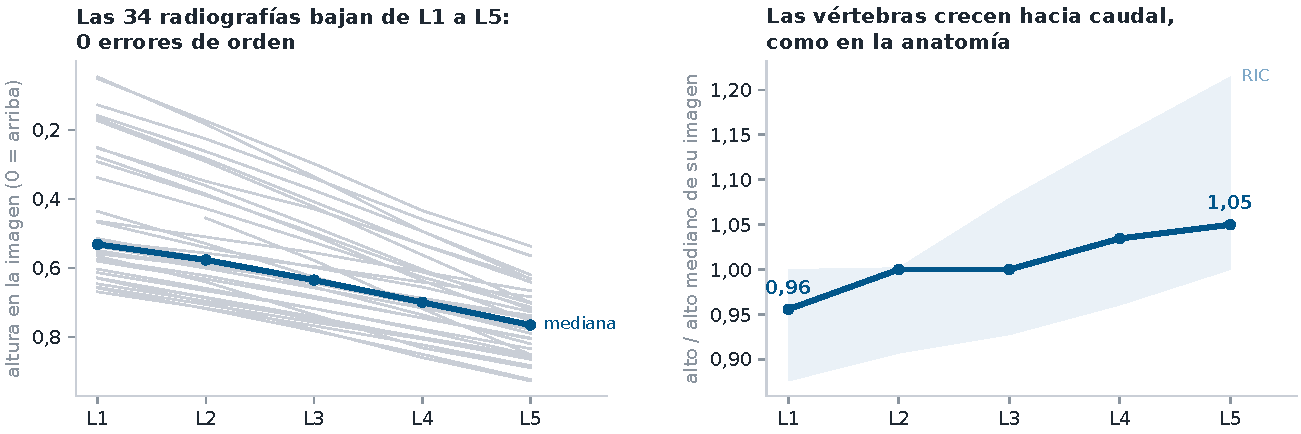
\includegraphics[height=4.3cm]{fig/anatomia.pdf}\\[0.6ex]
  \begin{columns}[T]
    \begin{column}{0.47\textwidth}
      \small
      \textbf{Orden craneocaudal:} el centroide vertical debe crecer de L1 a L5. Detecta \textbf{etiquetas intercambiadas} entre vecinas, algo que ningún método estadístico genérico ve.\\
      Resultado: \textbf{0 violaciones}.
    \end{column}
    \begin{column}{0.47\textwidth}
      \small
      \textbf{Progresión de tamaño:} el alto relativo crece de 0{,}96 (L1) a 1{,}05 (L5), coherente con el aumento del cuerpo vertebral hacia caudal: las anotaciones son \textbf{anatómicamente plausibles}.
    \end{column}
  \end{columns}
\end{frame}

\begin{frame}{NHANES: los 1.709 «errores» eran imágenes giradas}{Las mismas reglas de dominio, sobre 22.185 cajas}
  \begin{columns}[T]
    \begin{column}{0.52\textwidth}
      \footnotesize
      \begin{itemize}\setlength{\itemsep}{0.6ex}
        \item \textbf{Duplicados:} 36 imágenes con una vértebra repetida; se conserva la caja más cerca de la posición típica.
        \item \textbf{Primer intento del control de orden:} marcó \textcolor{alerta}{\textbf{1.709 cajas}}. Al revisarlas, no eran errores: eran \textbf{radiografías giradas 90° o invertidas}.
        \item \textbf{Rediseño:} primero se detecta la \textbf{orientación} (hacia dónde se extiende la columna) y después se exige un orden monótono \textbf{a lo largo del eje}, en cualquier sentido.
        \item Resultado: \textbf{26 cajas en 13 imágenes} son errores reales (p.\,ej. L1 y L2 con la misma caja).
      \end{itemize}
    \end{column}
    \begin{column}{0.45\textwidth}
      \centering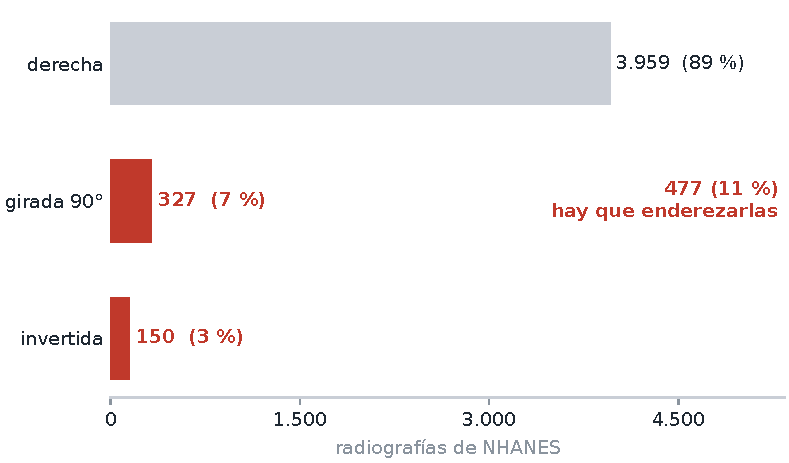
\includegraphics[height=3.9cm]{fig/tab_orientacion.pdf}\\[0.2ex]
      \begin{block}{Para el detector}
        \footnotesize Un 11\,\% de NHANES está girada o invertida: hay que \textbf{normalizar la orientación} antes de entrenar.
      \end{block}
    \end{column}
  \end{columns}
\end{frame}

% ===================================================================== OLTP
\separador[4]{OpenCV y exploración}

\begin{frame}{La inclinación de cada vértebra sale de su contorno}{Recomendación del docente: \texttt{cv2.moments} (tutorial de momentos de OpenCV)}
  \begin{columns}[c]
    \begin{column}{0.5\textwidth}
      \footnotesize
      \renewcommand{\arraystretch}{1.25}
      \begin{tabular}{@{}ll@{}}
        \toprule
        Descriptor & Cálculo \\ \midrule
        Área & $m_{00}$ \\
        Centroide & $(m_{10}/m_{00},\; m_{01}/m_{00})$ \\
        \textbf{Inclinación} & $\theta = \tfrac12\,\mathrm{atan2}(2\mu_{11},\, \mu_{20} - \mu_{02})$ \\
        Excentricidad & $\sqrt{1 - \lambda_2/\lambda_1}$ (autovalores de $\mu$) \\
        Circularidad & $4\pi A / P^2$ (\texttt{arcLength}) \\
        Solidez & $A / A_{\text{casco}}$ (\texttt{convexHull}) \\
        Hu 1, Hu 2 & \texttt{HuMoments}, escala log \\ \bottomrule
      \end{tabular}\\[1ex]
      \small
      \textbf{Validación:} $m_{00}$ coincide con el área por fórmula de Gauss (diferencia máxima $1{,}6\times10^{-6}$).\\[0.6ex]
      \textbf{Cobb aproximado} = máx $-$ mín de la inclinación de L1–L5 en la imagen, la lógica del ángulo de Cobb.
    \end{column}
    \begin{column}{0.48\textwidth}
      \centering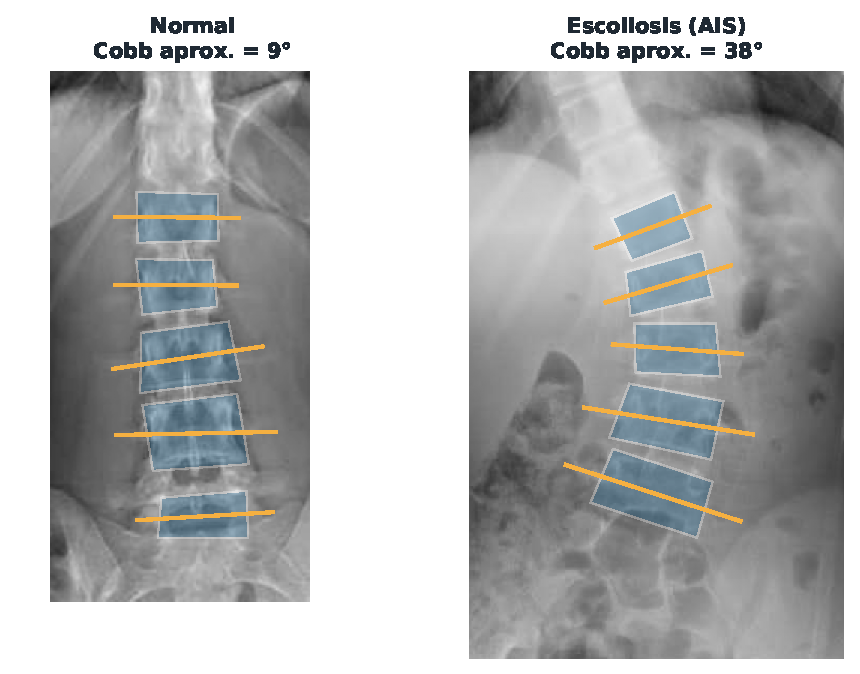
\includegraphics[height=5.6cm]{fig/momentos.pdf}\\
      {\scriptsize En naranja, el eje principal de cada vértebra.}
    \end{column}
  \end{columns}
\end{frame}

\begin{frame}{41 de 50 radiografías son grises guardadas como RGB}{Formato de píxel y nuevas columnas}
  \begin{columns}[T]
    \begin{column}{0.48\textwidth}
      \textbf{\color{itba}Metadatos de la imagen} (\texttt{cv2.imread(…, IMREAD\_UNCHANGED)})\\[0.6ex]
      \small
      \begin{itemize}\setlength{\itemsep}{0.4ex}
        \item 50 JPG, \textbf{3 canales, 8 bits}.
        \item 41 de 50 son radiografías en \textbf{gris guardadas como RGB} (los tres canales iguales).
        \item 50 resoluciones distintas: de 144$\times$606 a 1669$\times$3246 px.
        \item Formato, canales, profundidad de bits, tamaño y \textbf{vista} pasan a la tabla \texttt{imagen}.
      \end{itemize}
      \vspace{0.6ex}
      \textbf{\color{itba}Píxeles dentro de cada vértebra}\\[0.4ex]
      Máscara con \texttt{cv2.fillPoly}: \textbf{intensidad media} y \textbf{contraste} (desvío), en [0, 1].
    \end{column}
    \begin{column}{0.48\textwidth}
      \textbf{\color{itba}Columnas nuevas en los hechos}\\[0.6ex]
      \small
      \texttt{inclinacion}, \texttt{excentricidad}, \texttt{circularidad}, \texttt{solidez}, \texttt{hu1}, \texttt{hu2}, \texttt{intensidad\_media}, \texttt{contraste}\\[1ex]
      \textbf{\color{itba}Nuevo grano: segmento intervertebral}\\[0.6ex]
      L1–L2, L2–L3, L3–L4, L4–L5 por imagen (135 segmentos): ángulo segmentario, desplazamiento y separación entre vecinas.\\[1ex]
      \begin{block}{Sobre la torsión (\emph{twist})}
        \footnotesize La rotación axial no se mide en una radiografía 2D (requiere pedículos o tomografía). Los momentos miden la \textbf{inclinación} en el plano, base del ángulo de Cobb.
      \end{block}
    \end{column}
  \end{columns}
\end{frame}

\begin{frame}{P5 · Los momentos separan escoliosis (36°) y normales (7°)}{¿Los momentos de imagen detectan la patología?}
  \centering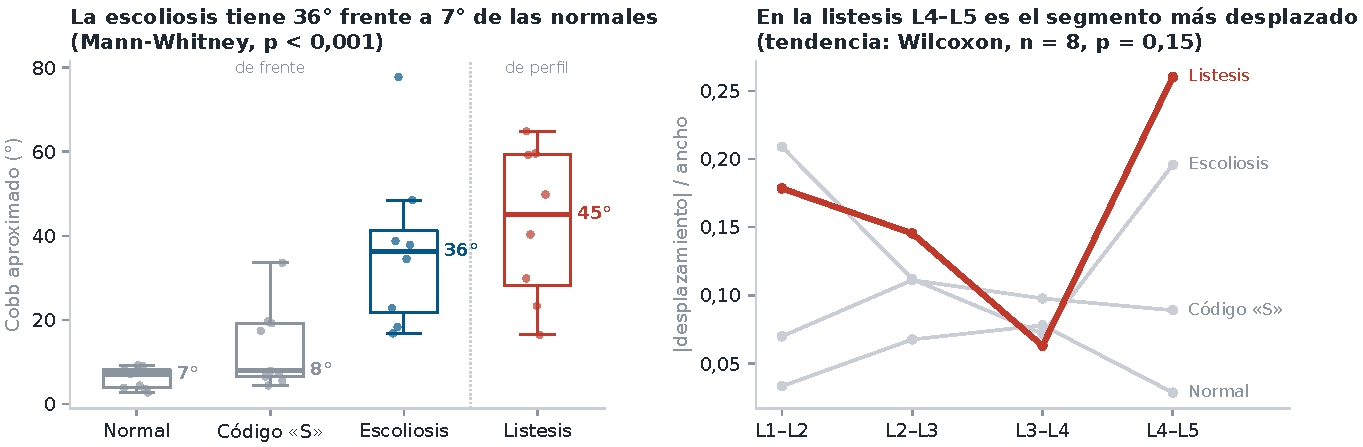
\includegraphics[height=4.0cm]{fig/p5.pdf}\\[0.4ex]
  \begin{columns}[T]
    \begin{column}{0.5\textwidth}
      \small
      \textbf{Vista:} escoliosis, normales y «S» son \textbf{de frente} (mide la curva); las listesis, \textbf{de perfil} (mide la lordosis).\\[0.4ex]
      \textbf{Escoliosis vs. normales:} Cobb mediano \textbf{36° vs. 7°}; Mann-Whitney $p < 0{,}001$.
    \end{column}
    \begin{column}{0.47\textwidth}
      \small
      \textbf{Listesis:} L4–L5 es el nivel más desplazado, pero \textbf{no significativo} frente al resto (Wilcoxon, $n = 8$, $p = 0{,}15$): tendencia.\\[0.4ex]
      {\color{itba}\textbf{Para el CDSS:} los contornos ya miden alineación.}
    \end{column}
  \end{columns}
\end{frame}

\begin{frame}{Exploratorio (1): la forma no da el nivel, sí la vista}{ACP de 12 descriptores estandarizados · 169 vértebras de Lumbar Spine}
  \centering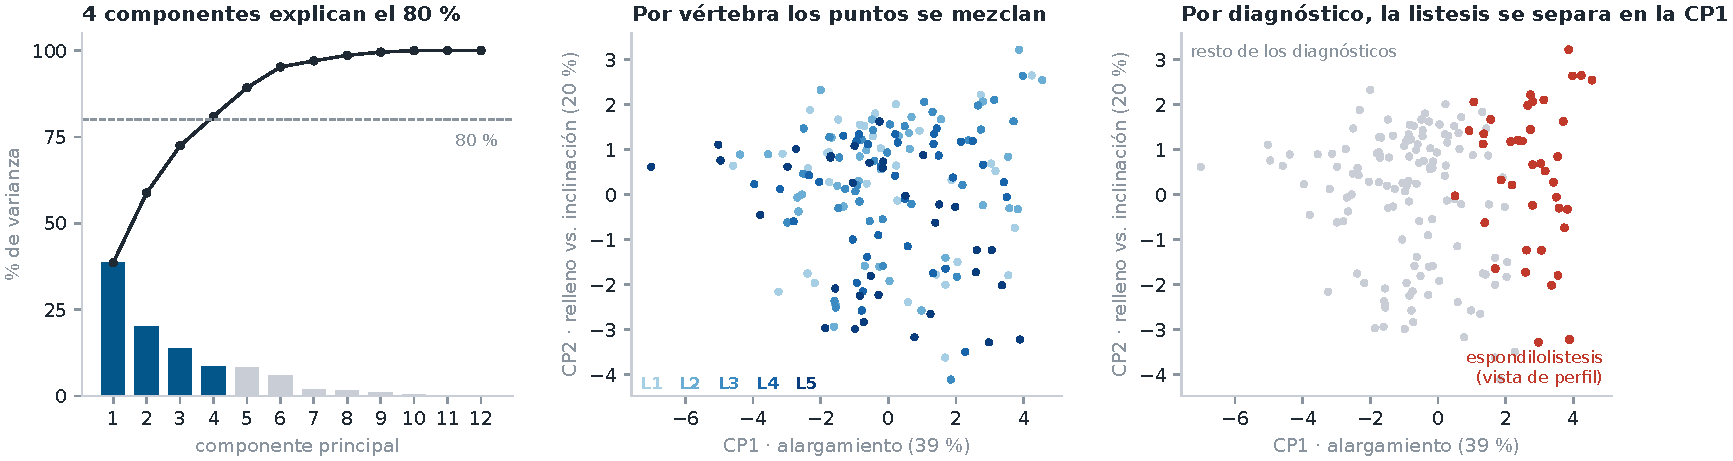
\includegraphics[width=\linewidth]{fig/eda_acp.pdf}\\[0.3ex]
  \begin{columns}[T]
    \begin{column}{0.48\textwidth}
      \small
      \textbf{4 componentes} explican el 80\,\%: CP1 es el \textbf{alargamiento} y CP2 el \textbf{relleno frente a la inclinación}.
    \end{column}
    \begin{column}{0.48\textwidth}
      \small
      Por vértebra los puntos \textbf{se mezclan}: el nivel lo da la \textbf{posición} (P3), no la forma. Por diagnóstico, la \textcolor{alerta}{\textbf{espondilolistesis}} se separa sobre la CP1.
    \end{column}
  \end{columns}
\end{frame}

\begin{frame}{Exploratorio (2): cuatro descriptores miden lo mismo}{Correlación de Spearman y distancia entre vectores de medias, como en el TP3}
  \centering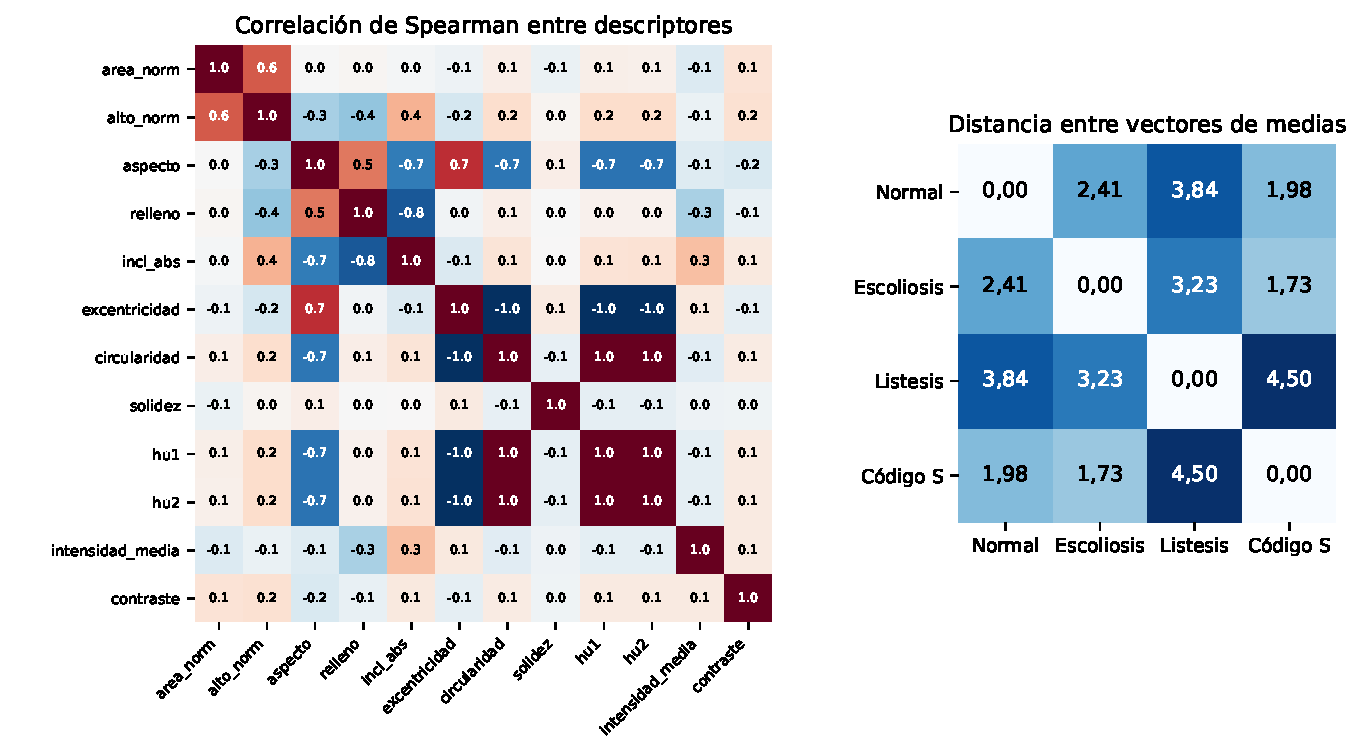
\includegraphics[height=4.75cm]{fig/eda_perfiles.pdf}\\[0.1ex]
  \begin{columns}[T]
    \begin{column}{0.48\textwidth}
      \footnotesize
      Excentricidad, circularidad, Hu1 y Hu2 tienen $|\rho| = 1$: miden lo mismo, \textbf{alcanza con una}.
    \end{column}
    \begin{column}{0.48\textwidth}
      \footnotesize
      La \textbf{listesis} es el perfil más lejano a la columna normal (3,84): vértebras más redondeadas, por la \textbf{vista de perfil}. El código «S» queda cerca de la escoliosis (1,73).
    \end{column}
  \end{columns}
\end{frame}

\separador[5]{Base de datos transaccional}

\begin{frame}{Siete tablas, dos con claves compuestas}{Modelo entidad-relación de la base transaccional (SQLite)}
  \centering
  \resizebox{\linewidth}{!}{%
  \begin{tikzpicture}[node distance=0.5cm]
    \tab{dataset}{(0,2.6)}{\textbf{PK} dataset\_id\\nombre, fuente, version\\licencia, sha256}
    \tab{diagnostico}{(0,0)}{\textbf{PK} diagnostico\_id\\nombre}
    \tab[3.2cm]{imagen}{(4.1,1.3)}{\textbf{PK} imagen\_id\\\textbf{FK} dataset\_id\\\textbf{FK} diagnostico\_id\\archivo, split, vista, orientación\\ancho\_px, alto\_px, anotada\\formato, canales, bits, tamaño\\sexo, edad, nivel\_listesis}
    \tab[3.3cm]{anotacion}{(8.4,1.3)}{\textbf{PK,FK} imagen\_id\\\textbf{PK,FK} vertebra\_id\\es\_atipico\\orden\_coherente\\motivo\_atipico\\geometria}
    \tab[3.3cm]{vertice}{(12.6,1.3)}{\textbf{PK,FK} imagen\_id\\\textbf{PK,FK} vertebra\_id\\\textbf{PK} orden\\x\_px, y\_px}
    \tab{vertebra}{(8.4,-1.6)}{\textbf{PK} vertebra\_id\\codigo, orden\_craneocaudal\\\textbf{FK} region\_id}
    \tab{region}{(4.1,-1.6)}{\textbf{PK} region\_id\\nombre}
    \draw[rel] (dataset.east) -- (imagen.west |- dataset.east) node[pos=0.5, above, font=\tiny, text=gris] {1:N};
    \draw[rel] (diagnostico.east) -- (imagen.west |- diagnostico.east) node[pos=0.5, above, font=\tiny, text=gris] {1:N};
    \draw[rel] (imagen.east) -- (anotacion.west) node[midway, above, font=\tiny, text=gris] {1:N};
    \draw[rel] (anotacion.east) -- (vertice.west) node[midway, above, font=\tiny, text=gris] {1:N};
    \draw[rel] (vertebra.north) -- (anotacion.south) node[midway, right, font=\tiny, text=gris] {1:N};
    \draw[rel] (region.east) -- (vertebra.west) node[midway, above, font=\tiny, text=gris] {1:N};
  \end{tikzpicture}}\\[0.8ex]
  {\footnotesize Una sola clave por tabla. \texttt{anotacion} y \texttt{vertice} usan \textbf{claves compuestas} formadas por las tablas que conectan.}
\end{frame}

\begin{frame}{Por qué está en tercera forma normal}
  \begin{columns}[T]
    \begin{column}{0.32\textwidth}
      \begin{block}{1FN — atomicidad}
        \footnotesize El polígono es una lista de largo variable (\textbf{grupo repetitivo}). Guardarlo como texto violaría la atomicidad: cada vértice es una fila de \texttt{vertice}.
      \end{block}
    \end{column}
    \begin{column}{0.32\textwidth}
      \begin{block}{2FN — sin dependencias parciales}
        \footnotesize Con clave \texttt{(imagen\_id, vertebra\_id)}, la resolución o el sexo dependen sólo de la imagen y viven en \texttt{imagen}; el código y el orden, sólo de la vértebra. En \texttt{anotacion} quedan las marcas de calidad, que dependen del par.
      \end{block}
    \end{column}
    \begin{column}{0.32\textwidth}
      \begin{block}{3FN — sin transitivas}
        \footnotesize La región depende de la vértebra (\texttt{region}); el nombre del diagnóstico, de su id (\texttt{diagnostico}); la licencia y el hash, del dataset.
      \end{block}
    \end{column}
  \end{columns}
  \vspace{1.5ex}
  \small
  \begin{itemize}\setlength{\itemsep}{0.3ex}
    \item \textbf{No se guardan derivados} (caja, área): se calculan desde los vértices al cargar el almacén.
    \item Claves foráneas activas y \texttt{foreign\_key\_check}: \textbf{0 violaciones}; \texttt{CHECK} sobre \texttt{split}, \texttt{sexo}, \texttt{edad}.
  \end{itemize}
\end{frame}

% ===================================================================== DW
\separador[6]{Almacén de datos}

\begin{frame}{Copo de nieve con dos tablas de hechos}{Constelación de hechos: comparten dimensiones, cada una con su grano}
  \centering
  \resizebox{!}{5.2cm}{%
      \begin{tikzpicture}
        \node[hechos=3.7cm] (f) at (0,1.9) {\textcolor{white}{\textbf{fact\_vertebra\_anotada}}\nodepart{two}\textbf{PK,FK} imagen\_key\\\textbf{PK,FK} vertebra\_key\\[0.3ex]area\_norm, alto\_norm, aspecto, relleno\\cy\_rel, \textbf{inclinacion}, excentricidad\\circularidad, solidez, hu1, hu2\\intensidad\_media, contraste\\es\_atipico, orden\_coherente, geometria};
        \node[hechos=3.7cm] (fs) at (0,-2.2) {\textcolor{white}{\textbf{fact\_segmento}}\nodepart{two}\textbf{PK,FK} imagen\_key\\\textbf{PK,FK} segmento\_key\\[0.3ex]delta\_inclinacion\\desplazamiento\_rel\\separacion\_rel};
        \node[tabla=3.4cm, anchor=west] (di) at (4.6,0) {\textcolor{white}{\textbf{dim\_imagen}}\nodepart{two}\textbf{PK} imagen\_key\\split, resolucion, vista\\orientacion, formato, bits\\sexo, edad, grupo\_edad\\anotada, completa\\\textbf{FK} dataset\_key\\\textbf{FK} diagnostico\_key};
        \node[tabla=2.6cm, anchor=west] (dd) at (8.6,1.4) {\textcolor{white}{\textbf{dim\_dataset}}\nodepart{two}\textbf{PK} dataset\_key\\nombre, licencia\\(2 fuentes)};
        \node[tabla=2.6cm, anchor=west] (dg) at (8.6,-1.4) {\textcolor{white}{\textbf{dim\_diagnostico}}\nodepart{two}\textbf{PK} diagnostico\_key\\nombre};
        \node[tabla=2.9cm, anchor=east] (dv) at (-2.9,1.9) {\textcolor{white}{\textbf{dim\_vertebra}}\nodepart{two}\textbf{PK} vertebra\_key\\codigo, orden\\\textbf{FK} region\_key};
        \node[tabla=2.9cm, anchor=east] (ds) at (-2.9,-2.2) {\textcolor{white}{\textbf{dim\_segmento}}\nodepart{two}\textbf{PK} segmento\_key\\nombre (L1-L2 …)\\\textbf{FK} vertebra\_sup\_key\\\textbf{FK} vertebra\_inf\_key};
        \node[tabla=2.3cm, anchor=south] (dr) at ([yshift=0.7cm]dv.north) {\textcolor{white}{\textbf{dim\_region}}\nodepart{two}\textbf{PK} region\_key\\nombre};
        \draw[rel] (di.west) -- (f.east);
        \draw[rel] (di.west) -- (fs.east);
        \draw[rel] (dv.east) -- (f.west);
        \draw[rel] (ds.east) -- (fs.west);
        \draw[rel] (dv.south) -- (ds.north);
        \draw[rel] (dr.south) -- (dv.north);
        \draw[rel] (dd.west) -- ([yshift=0.5cm]di.east);
        \draw[rel] (dg.west) -- ([yshift=-0.5cm]di.east);
      \end{tikzpicture}}\\[0.8ex]
  {\scriptsize PK compuestas por las claves de sus dimensiones en ambas tablas de hechos · \texttt{dim\_segmento} se normaliza hacia \texttt{dim\_vertebra} · cervical o torácica = agregar filas · miembro «sin dato» · carga desde la base transaccional.}
\end{frame}

\begin{frame}{Cada métrica del almacén responde a una pregunta}
  \scriptsize
  \renewcommand{\arraystretch}{1.1}
  \begin{tabularx}{\linewidth}{@{}lXl@{}}
    \toprule
    Métrica / atributo & Cálculo en el ETL & Responde \\ \midrule
    \texttt{COUNT(*)} sobre hechos & cantidad de anotaciones & \textbf{\color{itba}P1} \\
    \texttt{dim\_imagen.completa} & 1 si la imagen tiene las 5 vértebras & \textbf{\color{itba}P1} \\
    \texttt{area\_norm} & área del polígono / mediana del área de las vértebras de la misma imagen & \textbf{\color{itba}P2}, \textbf{\color{itba}P3} \\
    \texttt{aspecto}, \texttt{relleno} & ancho/alto de la caja; área del polígono / área de la caja & \textbf{\color{itba}P2} \\
    \texttt{es\_atipico}, \texttt{motivo\_atipico} & marca de calidad (Tukey, Mahalanobis, orden) & \textbf{\color{itba}P2} \\
    \texttt{alto\_norm}, \texttt{cy\_rel} & alto relativo a sus vecinas; centroide vertical / alto de la imagen & \textbf{\color{itba}P3} \\
    \texttt{orden\_coherente} & 1 si respeta el orden L1$\rightarrow$L5 & \textbf{\color{itba}P3} \\
    diagnóstico, sexo, \texttt{grupo\_edad} & extraídos del nombre de archivo & \textbf{\color{itba}P4} \\
    \texttt{excentricidad}, \texttt{circularidad}, \texttt{solidez}, \texttt{hu1/2} & momentos del contorno (OpenCV) & \textbf{\color{itba}P2} \\
    \texttt{intensidad\_media}, \texttt{contraste} & píxeles dentro del polígono (máscara OpenCV) & \textbf{\color{itba}P2} \\
    \texttt{inclinacion}; Cobb aproximado & eje principal por momentos; \texttt{MAX $-$ MIN} por imagen en la consulta & \textbf{\color{itba}P5} \\
    \texttt{delta\_inclinacion}, \texttt{desplazamiento\_rel}, \texttt{separacion\_rel} & en \texttt{fact\_segmento}: ángulo, deslizamiento y espacio entre vecinas & \textbf{\color{itba}P5} \\ \bottomrule
  \end{tabularx}
\end{frame}

% ===================================================================== resultados
\separador[7]{Resultados y veredicto}

\begin{frame}{Resultados: cinco preguntas, cinco respuestas}
  \begin{center}
    \dato{4.438}{completas L1–L5 (33 + 4.405)}\dato{1{,}03}{razón máx/mín entre clases}\dato{477}{radiografías giradas o invertidas}\dato{36°}{Cobb en escoliosis (7° normales)}
  \end{center}
  \vspace{0.3ex}
  \begin{columns}[T]
    \begin{column}{0.48\textwidth}
      \footnotesize
      \begin{itemize}\setlength{\itemsep}{0.3ex}
        \item \textbf{P1:} Lumbar Spine sola no alcanza; con NHANES, sí.
        \item \textbf{P2:} calidad alta; 5 contornos a revisar.
        \item \textbf{P3:} orden coherente; 11\,\% de NHANES girada o invertida.
        \item \textbf{P4:} escoliosis 17, «S» 16, normales 9, listesis 8; mayoría mujeres y menores de 18.
        \item \textbf{P5:} Cobb aproximado 36° en escoliosis vs. 7° en normales ($p < 0{,}001$).
      \end{itemize}
    \end{column}
    \begin{column}{0.48\textwidth}
      \centering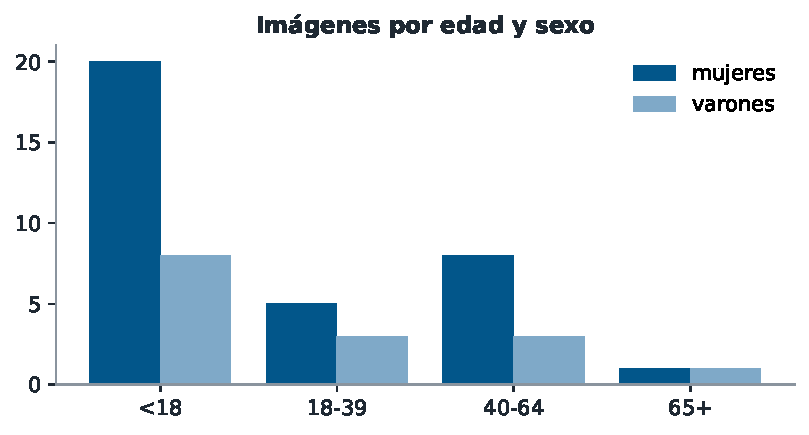
\includegraphics[width=0.95\linewidth]{fig/representatividad.pdf}
    \end{column}
  \end{columns}
\end{frame}

\begin{frame}{Veredicto: con NHANES alcanza, enderezando la orientación}
  \begin{columns}[c]
    \begin{column}{0.55\textwidth}
      \begin{block}{Respuesta a la pregunta de investigación}
        \small \textbf{Lumbar Spine sola no alcanza} (33 completas, 16\,\% del mínimo). \textbf{Sumando NHANES sí}: 4.438 imágenes completas, con dos condiciones: \textbf{normalizar la orientación} y \textbf{sumar vistas de frente}, que hoy sólo aporta Lumbar Spine.
      \end{block}
      \vspace{1ex}
      \small
      \textbf{Próximos pasos para la tesis:}
      \footnotesize
      \begin{enumerate}\setlength{\itemsep}{0.1ex}
        \item \textbf{Enderezar} las 477 radiografías de NHANES.
        \item \textbf{Entrenar} con NHANES; \textbf{validar} con Lumbar Spine.
        \item Revisar 5 contornos; anotar las 16 de escoliosis y «S».
        \item Usar los contornos para la \textbf{alineación} del SINS.
      \end{enumerate}
    \end{column}
    \begin{column}{0.42\textwidth}
      \small
      \textbf{Limitaciones}
      \footnotesize
      \begin{itemize}\setlength{\itemsep}{0.1ex}
        \item El código «S» no está documentado por la fuente.
        \item Los metadatos dependen de la convención del nombre de archivo.
        \item Imagen $\neq$ paciente: no hay identificador de paciente.
        \item Umbral de 200 imágenes: supuesto ajustable.
        \item NHANES: sólo perfil, cajas estiradas, sin metadatos.
        \item Vista inferida del diagnóstico; \emph{twist} no medible en 2D; $n \approx 8$ por grupo.
      \end{itemize}
    \end{column}
  \end{columns}
\end{frame}

% ===================================================================== IA
\begin{frame}{Uso de inteligencia artificial}
  \begin{columns}[T]
    \begin{column}{0.48\textwidth}
      \textbf{\color{itba}Declaración}\\[0.5ex]
      \scriptsize
      \begin{itemize}\setlength{\itemsep}{0.1ex}
        \item «Claude Sonnet 4.5» para «redacción de celdas Markdown de la primera versión».
        \item «ChatGPT 4.5» para «sugerir esquemas SQLite de la primera versión».
        \item «GitHub Copilot» para «autocompletar parsing YOLO y gráficos».
        \item «Claude Opus 5.5» para «reestructurar el notebook: extracción sin credenciales, control de calidad, modelos con claves compuestas y tablero».
        \item «Claude Opus 5.5» para «implementar los momentos de OpenCV recomendados por el docente, el formato de píxel, la tabla de segmentos e integrar NHANES como segunda fuente».
        \item «Claude Opus 5.5» para «aplicar storytelling a gráficos y diapositivas e integrar el informe en el notebook».
      \end{itemize}
    \end{column}
    \begin{column}{0.48\textwidth}
      \textbf{\color{itba}Human-in-the-loop: decisiones verificadas}\\[0.5ex]
      \footnotesize
      \begin{itemize}\setlength{\itemsep}{0.1ex}
        \item Hash del zip y \emph{Ejecutar todo} en una sesión nueva.
        \item Superposición de polígonos sobre la radiografía.
        \item Revisión manual del duplicado y de la tabla nombre $\rightarrow$ metadatos.
        \item Rechazo del área relativa a la imagen (49 falsos atípicos) y cambio a normalización por vecinas.
        \item $m_{00}$ = área de Gauss; revisión visual de la vista por diagnóstico.
        \item Detección del desbordamiento \texttt{int16}.
        \item 1.709 «errores de orden» en NHANES: revisados, eran imágenes giradas.
        \item Cada métrica contrastada con P1–P5; ejes de conteo sin decimales.
      \end{itemize}
    \end{column}
  \end{columns}
\end{frame}

{\setbeamertemplate{footline}{}
\begin{frame}[plain]
  \begin{tikzpicture}[remember picture, overlay]
    \fill[itba] (current page.south west) rectangle (current page.north east);
    \node[text=white, font=\Huge\bfseries] at ([yshift=1cm]current page.center) {¡Gracias!};
    \node[text=white, font=\large] at ([yshift=-0.1cm]current page.center) {Preguntas};
    \node[text=white, font=\footnotesize, align=center] at ([yshift=-1.6cm]current page.center)
      {\texttt{github.com/marcoskantor/Curso\_Introduccion\_Ingenieria\_Datos}\\[0.3ex]Proyecto\_final.ipynb · app.py · data/raw/};
  \end{tikzpicture}
\end{frame}}

% ===================================================================== anexo
\appendix
\separador{Anexo para el coloquio}

\begin{frame}[fragile]{A1 · Parsing y área del polígono}
  \begin{columns}[T]
    \begin{column}{0.55\textwidth}
\begin{lstlisting}[language=Python]
x = vals[0::2] * ancho_px   # desnormalizar
y = vals[1::2] * alto_px
area = 0.5 * abs(np.dot(x, np.roll(y, -1))
                 - np.dot(y, np.roll(x, -1)))
\end{lstlisting}
      \vspace{1ex}
      \small Fórmula de Gauss (\emph{shoelace}):
      \[ A = \tfrac{1}{2}\Big|\textstyle\sum_{i=1}^{n} (x_i\,y_{i+1} - y_i\,x_{i+1})\Big| \]
      con $x_{n+1} = x_1$; \texttt{np.roll} implementa el índice cíclico.
    \end{column}
    \begin{column}{0.42\textwidth}
      \small
      \begin{itemize}\setlength{\itemsep}{0.5ex}
        \item 4 valores $\Rightarrow$ caja \texttt{xc yc w h}: se convierte a sus 4 esquinas.
        \item Número impar o $<$ 6 valores $\Rightarrow$ se \textbf{rechaza} la línea y se registra.
        \item Caja envolvente = mín/máx de los vértices; centroide = media de los vértices.
        \item \texttt{relleno} = área del polígono / área de la caja: 1 si el contorno es un rectángulo.
      \end{itemize}
    \end{column}
  \end{columns}
\end{frame}

\begin{frame}[fragile]{A2 · Tukey y Mahalanobis robusta}
  \begin{columns}[T]
    \begin{column}{0.52\textwidth}
\begin{lstlisting}[language=Python]
q1, q3 = g[var].quantile([0.25, 0.75])
lo = q1 - 2.0 * (q3 - q1)
hi = q3 + 2.0 * (q3 - q1)

rel = np.log(X / X.groupby(vertebra).median())
z   = (rel - rel.median()) / MAD(rel)
d2  = z @ inv(cov(z)) @ z.T     # por fila
atipico = d2 > chi2.ppf(0.999, 3)  # 16.27
\end{lstlisting}
    \end{column}
    \begin{column}{0.45\textwidth}
      \small
      \begin{itemize}\setlength{\itemsep}{0.6ex}
        \item \textbf{¿Por qué Tukey y no $z$?} Shapiro–Wilk rechaza normalidad en 10 de 15 casos: $\pm 3\sigma$ supone normalidad; los cuartiles no.
        \item \textbf{¿Por qué $k=2$?} Más conservador que 1{,}5: con $n \approx 34$ por vértebra se evita marcar variación anatómica normal.
        \item \textbf{¿Por qué robusta?} Media y desvío se contaminan con los propios atípicos; mediana y MAD no.
        \item \textbf{¿Por qué logaritmo?} Las razones son asimétricas (0{,}5 y 2 están a la misma distancia de 1).
      \end{itemize}
    \end{column}
  \end{columns}
\end{frame}

\begin{frame}[fragile]{A3 · Orden craneocaudal y regla de duplicados}
  \begin{columns}[T]
    \begin{column}{0.53\textwidth}
\begin{lstlisting}[language=Python]
# duplicados: el mas cercano a la posicion esperada
anot["dist"] = (anot.cy_rel
    - anot.vertebra.map(mediana_cy)).abs()
anot = (anot.sort_values("dist")
        .drop_duplicates(["archivo", "vertebra"]))

# orden: cy debe crecer de L1 a L5
prev = anot.groupby("archivo").cy_rel.shift(1)
nxt  = anot.groupby("archivo").cy_rel.shift(-1)
roto = (prev.notna() & (anot.cy_rel <= prev)) | \
       (nxt.notna()  & (anot.cy_rel >= nxt))
\end{lstlisting}
    \end{column}
    \begin{column}{0.44\textwidth}
      \small
      \begin{itemize}\setlength{\itemsep}{0.6ex}
        \item La posición vertical se normaliza por el alto de la imagen ($c_y$/alto) para comparar imágenes.
        \item La mediana por vértebra es el «lugar esperado» de esa vértebra.
        \item El control de orden compara cada vértebra con sus vecinas en la misma imagen (\texttt{shift} dentro del grupo).
        \item Supuesto: radiografías con la columna vertical (se verificó visualmente).
      \end{itemize}
    \end{column}
  \end{columns}
\end{frame}

\begin{frame}[fragile]{A4 · Carga del almacén desde la base transaccional}
  \begin{columns}[T]
    \begin{column}{0.56\textwidth}
\begin{lstlisting}[language=SQL]
ATTACH DATABASE 'spine_oltp.db' AS oltp;
INSERT INTO dim_imagen
SELECT i.imagen_id, i.archivo, i.split, ...,
       COALESCE(i.sexo, 'sin dato'),
       CASE WHEN i.edad < 18 THEN '<18' ... END,
       COUNT(a.vertebra_id),
       CASE WHEN COUNT(a.vertebra_id) = 5
            THEN 1 ELSE 0 END,           -- completa
       COALESCE(i.diagnostico_id, 0)    -- miembro "sin dato"
FROM oltp.imagen i
LEFT JOIN oltp.anotacion a USING (imagen_id)
GROUP BY i.imagen_id;
\end{lstlisting}
    \end{column}
    \begin{column}{0.41\textwidth}
      \small
      \begin{itemize}\setlength{\itemsep}{0.6ex}
        \item \texttt{LEFT JOIN}: las imágenes sin anotar también entran a la dimensión (P1 las necesita).
        \item Hechos: métricas recalculadas desde \texttt{vertice}, la fuente de verdad.
        \item \texttt{area\_norm} y \texttt{alto\_norm} se calculan con la mediana \textbf{por imagen} (\texttt{groupby + transform}).
        \item Validación: conteos por tabla y \texttt{PRAGMA foreign\_key\_check}.
      \end{itemize}
    \end{column}
  \end{columns}
\end{frame}

\begin{frame}[fragile]{A5 · Momentos y Cobb aproximado}
  \begin{columns}[T]
    \begin{column}{0.55\textwidth}
\begin{lstlisting}[language=Python]
cnt = np.column_stack([x, y]).astype(np.float32)
m = cv2.moments(cnt.reshape(-1, 1, 2))
mu20 = m["mu20"] / m["m00"]
mu02 = m["mu02"] / m["m00"]
mu11 = m["mu11"] / m["m00"]
theta = 0.5 * np.degrees(np.arctan2(2*mu11, mu20 - mu02))
\end{lstlisting}
\begin{lstlisting}[language=SQL]
SELECT imagen_key,
       MAX(inclinacion) - MIN(inclinacion) AS cobb_aprox
FROM fact_vertebra_anotada
GROUP BY imagen_key HAVING COUNT(*) >= 4;
\end{lstlisting}
    \end{column}
    \begin{column}{0.42\textwidth}
      \small
      \begin{itemize}\setlength{\itemsep}{0.5ex}
        \item Los momentos centrales $\mu_{pq}$ son la «covarianza» del contorno: su eje principal es la dirección de máxima dispersión.
        \item Divididos por $m_{00}$ no dependen del tamaño de la vértebra.
        \item \texttt{atan2} resuelve el cuadrante; el ½ viene de la fórmula del ángulo doble.
        \item Pruebas no paramétricas porque $n \approx 8$ y no hay normalidad.
      \end{itemize}
    \end{column}
  \end{columns}
\end{frame}

\end{document}
